\chapter{Разработка программного обеспечения для численного моделирования}

Для проведения комплексного численного исследования динамики опухолевых
процессов, формализованных в предыдущей главе, было разработано
специализированное программное обеспечение. Программный комплекс спроектирован
как инструмент, объединяющий вычислительное ядро, модуль глобальной оптимизации
и интерактивный графический интерфейс для анализа результатов в режиме реального времени.

\section{Обоснование выбора стека технологий и архитектурных решений
программного комплекса}

Выбор технологического стека определялся необходимостью интеграции методов
высокопроизводительных вычислений с гибкими средствами визуализации. В качестве
основного языка реализации выбран Python 3.10. Данное решение обусловлено не
только развитой экосистемой научных библиотек, но и возможностью использования
высокоуровневых интерфейсов для управления сложными алгоритмами, что критически
важно при автоматизации калибровки математических моделей на основе клинических данных.

Математический фундамент системы реализован на базе пакета SciPy \cite{scipy}, в частности
модуля \texttt{integrate}. Для решения систем обыкновенных дифференциальных
уравнений применен метод Дормана-Принса (RK45) \cite{dormand_prince}. В отличие от классического
метода Рунге-Кутты 4-го порядка с фиксированным шагом, алгоритм RK45 обладает
адаптивным контролем локальной погрешности. Это позволяет программному
обеспечению автоматически корректировать вычислительную сетку: увеличивать шаг
на участках стагнации и минимизировать его в моменты терапевтического
воздействия, когда производные концентраций клеток претерпевают резкие
изменения. Для обеспечения высокой скорости векторных операций и эффективного
управления памятью при обработке массивов данных задействована библиотека NumPy \cite{numpy}.

Графический интерфейс был построен на базе фреймворка PyQt5, который
реализует событийно-ориентированную модель взаимодействия \cite{oop}. Это позволило
создать динамическую систему, в которой программный контроллер перехватывает
сигналы от элементов управления (слайдеров и кнопок) и мгновенно инициирует
циклы пересчета модели. Визуализация расчетных кривых осуществляется через
интеграцию Matplotlib в среду PyQt5.
Применение программного интерфейса библиотеки
Matplotlib \cite{matplotlib} позволяет расширить стандартные возможности визуализации за счет
поддержки интерактивного взаимодействия с осями графиков. Реализованный
функционал включает средства навигации по расчетным кривым и инструменты
экспорта изображений в векторные форматы, что гарантирует сохранение четкости
графического материала при любом уровне масштабирования

\section{Проектирование интерфейса и логики работы программного обеспечения}

Графический интерфейс разработанного программного комплекса реализован на базе
многовкладочной архитектуры, что позволяет разграничить задачи визуализации решения
системы дифференциальных уравнений математической модели и анализа
чувствительности параметров данной модели. Основное окно приложения
(рис. \ref{fig:gui_layout}) включает вкладку <<Визуализация модели>>,
предназначенную для интерактивного исследования динамики системы.

\subsection{Проектирование пользовательского интерфейса программного обеспечения}

Графический интерфейс разработанного программного обеспечения реализован на базе
многовкладочной архитектуры, что позволяет разграничить задачи оперативного
моделирования и глубокого параметрического анализа. Основное окно приложения
(рис. \ref{fig:gui_layout}) включает вкладку <<Визуализация модели>>,
предназначенную для интерактивного исследования динамики системы.

\begin{figure}[htbp]
  \centering
  
\includegraphics[width=0.8\textwidth]{gui_layout.png}
  \caption{Графический интерфейс программного обеспечения (вкладка визуализации модели)}
  \label{fig:gui_layout}
\end{figure}

В правой части окна расположена панель управления, содержащая блоки
параметров модели ($a, b, c, \mu, d, p, \lambda$) и начальных условий ($T_0,
I_0, C_0, t_{end}$), реализованные в виде интерактивных регуляторов
(слайдеров). Изменение любого параметра инициирует автоматический пересчет
системы ОДУ и обновление визуализации на главном холсте в логарифмическом
масштабе. Модуль визуализации поддерживает наложение экспериментальных
клинических данных с отображением доверительных интервалов и автоматическим
расчетом коэффициента детерминации $R^2$ для верификации математической модели.

Вторая вкладка интерфейса --- <<Параметрический анализ>> (рис.
\ref{fig:gui_layout_2}) --- спроектирована для проведения автоматизированных
вычислительных экспериментов. В отличие от основной вкладки, данная панель
управления ориентирована на настройку диапазонов варьирования параметров.
Пользователю предоставляется возможность выбора исследуемой величины и
определения границ её изменения, на основе которых система генерирует сетку
значений для проведения серии расчетов.

\begin{figure}[htbp]
  \centering
  
\includegraphics[width=0.8\textwidth]{gui_layout_2.png}
  \caption{Графический интерфейс программного обеспечения (вкладка
  параметрического анализа)}
  \label{fig:gui_layout_2}
\end{figure}

Область построения графиков на этой вкладке поддерживает два режима
отображения. В режиме одномерного анализа формируется семейство кривых,
позволяющее визуально оценить чувствительность модели к изменениям конкретного
коэффициента. В режиме многофакторного анализа интерфейс генерирует двумерные
тепловые карты, где интенсивность цвета соответствует значениям выбранной
целевой метрики, такой как суммарная опухолевая нагрузка или эффективность
терапии. Реализованная компоновка элементов позволяет исследователю быстро
переключаться между общим анализом устойчивости системы и детальной проработкой
конкретных клинических сценариев.

\subsection{UML-диаграмма последовательности основных сценариев взаимодействия
с программным обеспечением}

Для детального описания динамического взаимодействия компонентов системы во
времени используется диаграмма последовательности (UML Sequence Diagram) \cite{Fowler2004UML},
представленная на рисунке \ref{fig:uml_sequence}. Она иллюстрирует механизмы
обмена сообщениями между тремя ключевыми сущностями: Пользователем (Actor),
Графическим интерфейсом (GUI на базе PyQt5) и Вычислительным ядром (Solver на базе SciPy).

\begin{figure}[ht!]
  \centering
  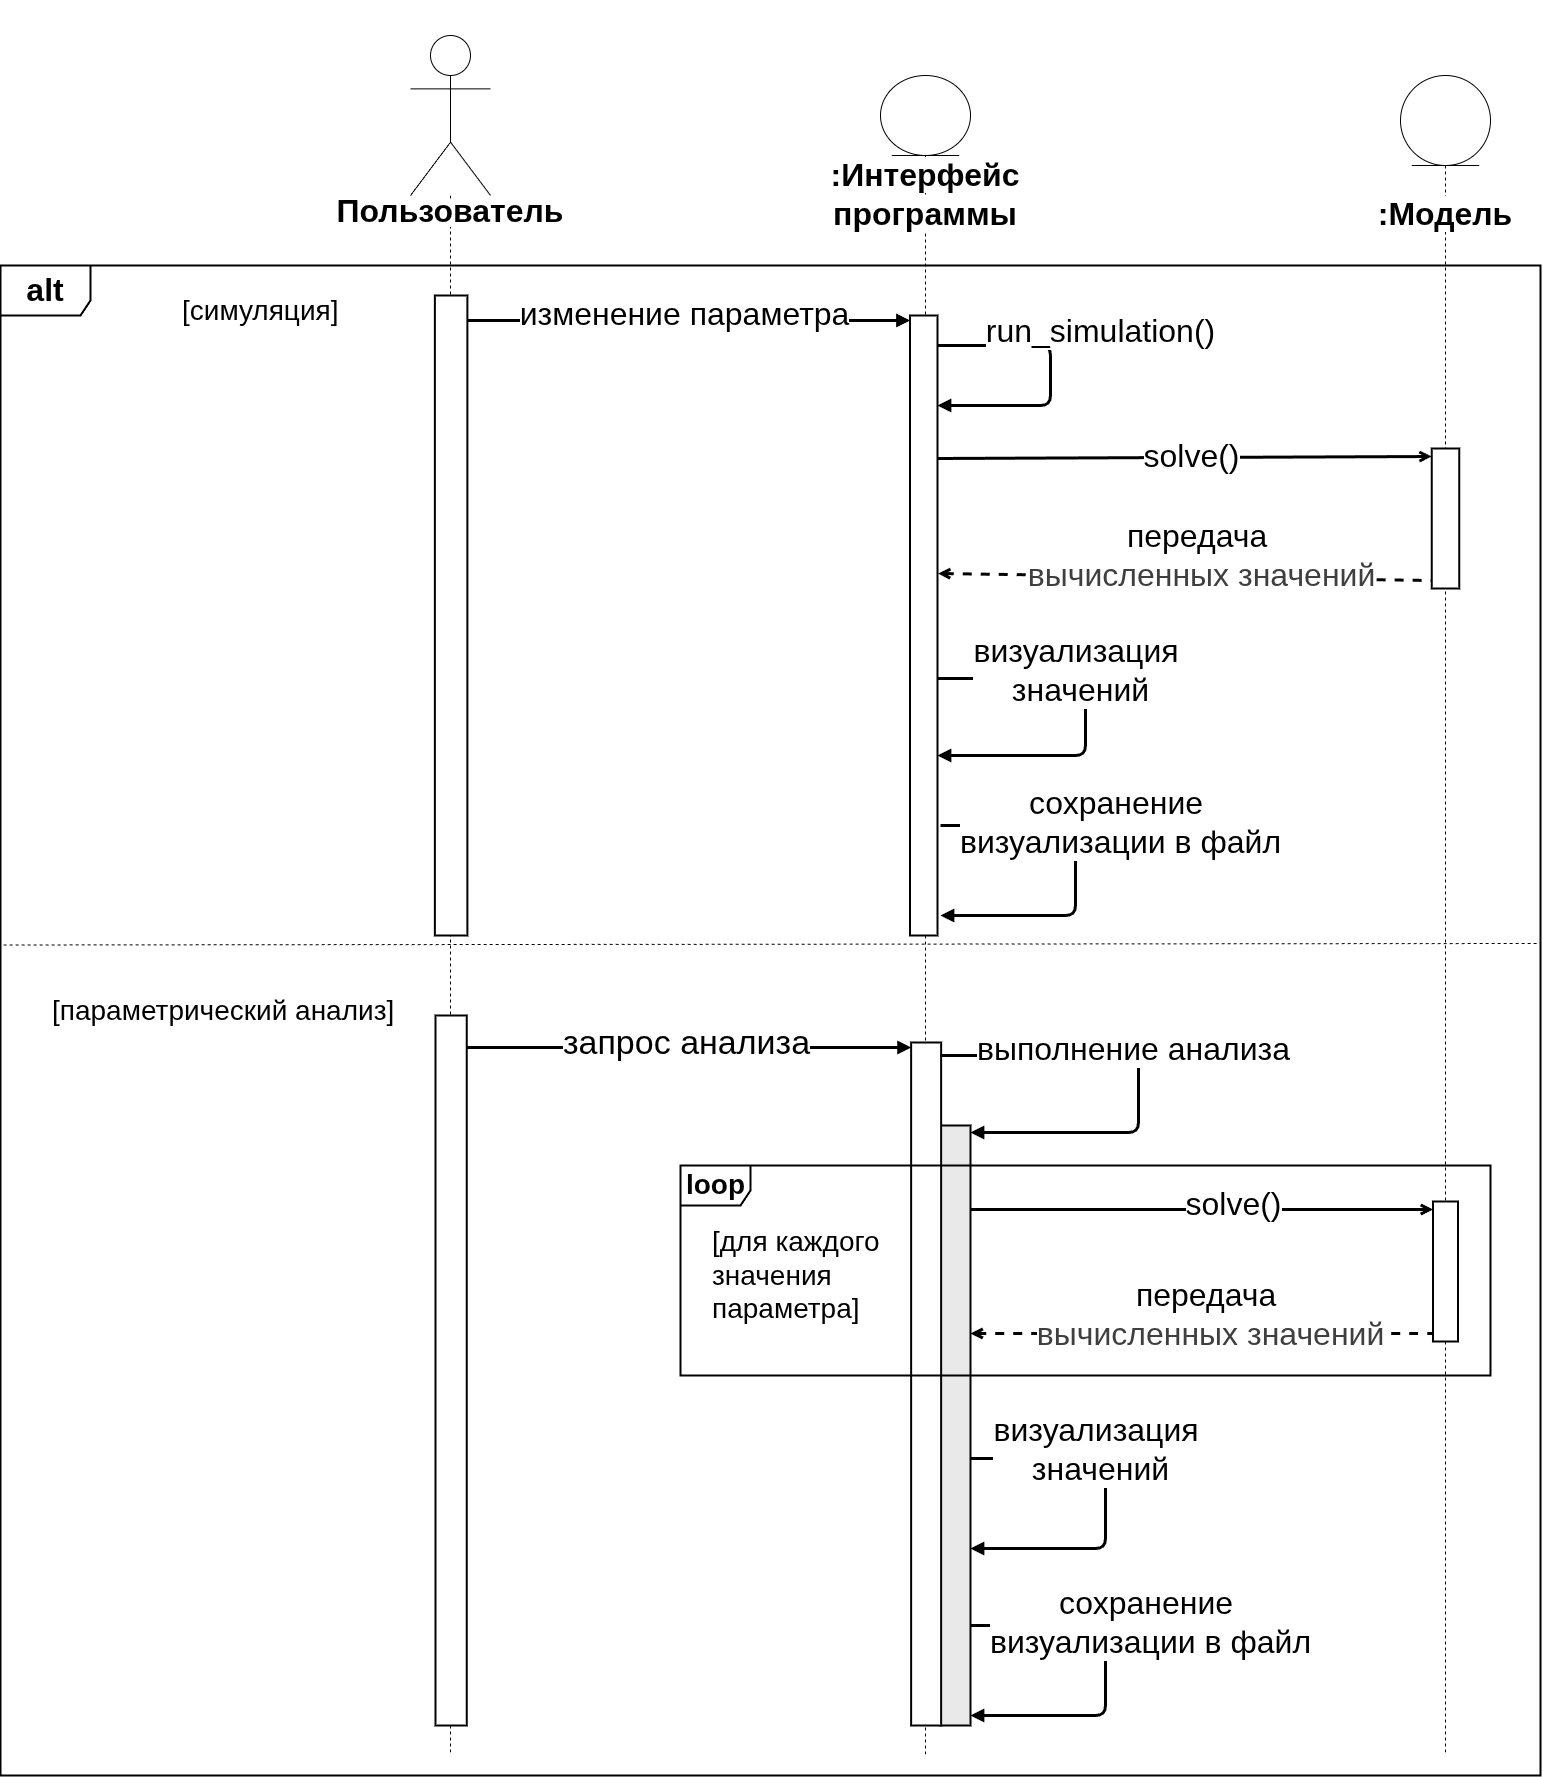
\includegraphics[width=0.9\textwidth]{fig/uml_sequence.png}
  \caption{Диаграмма последовательности основных сценариев работы:
  интерактивная симуляция и многопоточный анализ.}
  \label{fig:uml_sequence}
\end{figure}

Первый сценарий взаимодействия, описывающий интерактивную симуляцию,
инициируется пользователем в момент изменения положения любого из регуляторов
параметров или при выборе нового режима терапевтического воздействия. В ответ
на это действие графическая оболочка производит автоматический сбор актуальных
значений со всех элементов управления и передает их вычислительному модулю.
Внутри данного модуля запускается процедура численного решения системы
дифференциальных уравнений с использованием адаптивных методов интегрирования.

В ходе расчетов математическая модель определяет динамику изменения популяций
во времени и формирует результирующий набор данных, включающий временные метки
и соответствующие им концентрации клеток. Как только вычисления завершаются,
интерфейс обрабатывает полученные массивы, обновляя графические кривые и
пересчитывая показатели интегральной нагрузки на систему в режиме реального времени.

Второй сценарий, посвященный автоматизированному параметрическому анализу,
запускается при подтверждении пользователем команды на начало расчета в
соответствующем разделе программы. Логика этого процесса отличается повышенной
сложностью и включает в себя несколько последовательных этапов. Сразу после
запуска система временно ограничивает доступ к элементам ввода, что исключает
возникновение конфликтов при попытке повторного вызова процедур до завершения
текущих операций. Затем инициируется цикл многократных вычислений, в ходе
которого программная среда последовательно варьирует исследуемые параметры в
рамках заданной сетки.

Для каждого узла этой сетки модель выполняет полную симуляцию, а полученные
результаты используются для расчета специфических целевых показателей, таких
как пиковые нагрузки, темпы роста или суммарная токсичность. После прохождения
всех итераций накопленные данные трансформируются в итоговые визуальные формы
-- семейства кривых или многомерные тепловые карты. Завершающим этапом
выполнения сценария является восстановление активности элементов управления,
сигнализирующее о готовности системы к дальнейшей работе.

Данная архитектура взаимодействия обеспечивает строгую изоляцию математической
логики от визуального представления, что позволяет модифицировать систему
уравнений без изменения кода пользовательского интерфейса.

\section{Алгоритм идентификации параметров модели на основе метода
дифференциальной эволюции}

Для решения задачи идентификации параметров, в частности коэффициентов
взаимодействия клеток и скорости иммунного ответа, в модуль интегрирован
алгоритм дифференциальной эволюции \cite{diff_evo}. Использование этого стохастического метода
глобальной оптимизации позволяет эффективно исследовать многомерное
пространство параметров и избегать преждевременной сходимости в локальных минимумах.

Логика функционирования данного алгоритма в составе вычислительного ядра (рис.
\ref{fig:de_flowchart}) базируется на эволюционном подходе к минимизации
функции потерь \cite{rmse}. На этапе инициализации в рамках заданных биологических
ограничений (\textit{bounds}) формируется начальная популяция векторов,
представляющих собой наборы искомых коэффициентов. Последующий итерационный
процесс организован в рамках цикла поколений, который продолжается до
выполнения критерия останова или достижения требуемой точности аппроксимации.

\begin{figure}[ht!]
  \centering
  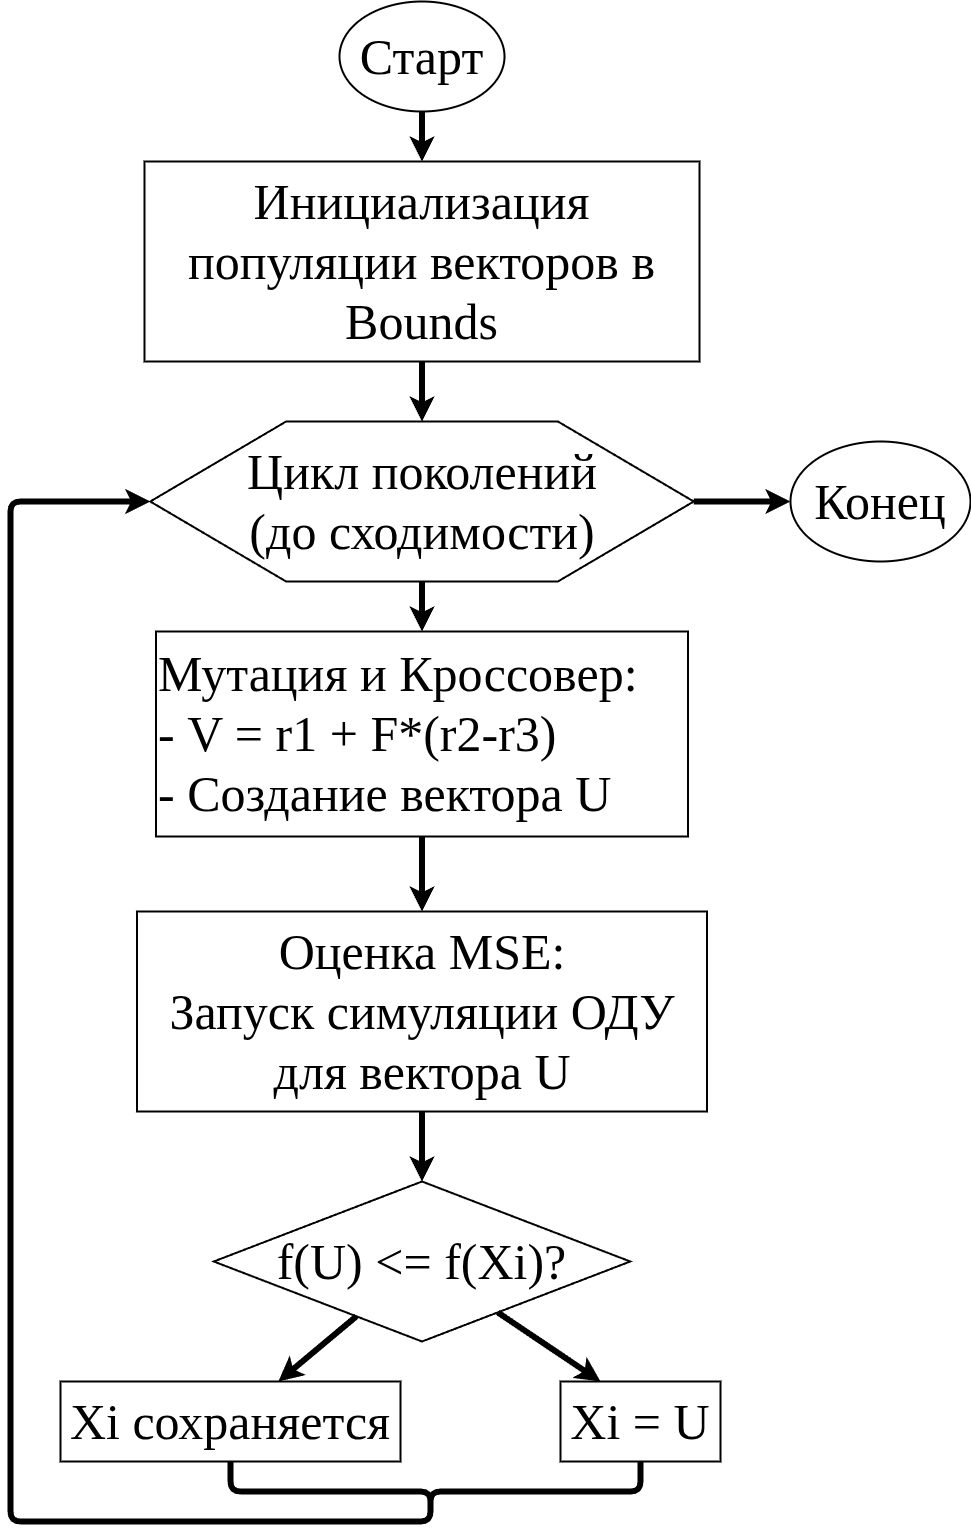
\includegraphics[width=0.4\textwidth]{fig/de_flowchart.png}
  \caption{Блок-схема алгоритма дифференциальной эволюции для калибровки
  параметров модели.}
  \label{fig:de_flowchart}
\end{figure}

На каждой итерации для целевых векторов выполняются процедуры мутации и
кроссовера. Путем комбинирования случайно выбранных векторов-доноров и
применения дифференциального веса $F$ формируется мутантный вектор, который
затем преобразуется в пробный вектор $U$. Критическим этапом алгоритма является
оценка пригодности (\textit{fitness evaluation}): вычислительный модуль
инициирует запуск симуляции системы ОДУ для параметров вектора $U$ и
рассчитывает среднеквадратичную ошибку (MSE) относительно экспериментальных данных.

Заключительный этап каждой итерации — селекция — основан на сравнении значений
целевой функции пробного вектора $f(U)$ и текущего вектора $f(X_i)$. Если новый
набор параметров обеспечивает меньшую или равную ошибку, он замещает текущий
вектор в популяции следующего поколения; в противном случае сохраняется
исходное состояние. Такая циклическая архитектура обеспечивает
автоматизированную и физически интерпретируемую калибровку модели, адаптируя
теоретическую систему уравнений под индивидуальную динамику конкретных
клинических случаев.